\documentclass[12pt]{article}
\usepackage{graphicx}
\usepackage{amsmath}
\begin{center}
\textbf{Pritish Prakash Salunke}
\end{center}
\hline
\label{sec:PritishPrakashSalunke}
\begin{document}
\begin{flushleft}
14,Royal row houses,\hspace{2in} Contact:9765490931\\ 
Opp.glass factory,\hspace{1in} Email Id:pritish.p.salunke.004@gmail.com \\ 
Wadala-Pathardi road,\\
Indira nagar,\\ 
Nashik-422009,\\ 
Maharashtra.
\vspace{-4ex}
\begin{figure}[h]
	\begin{flushright}
		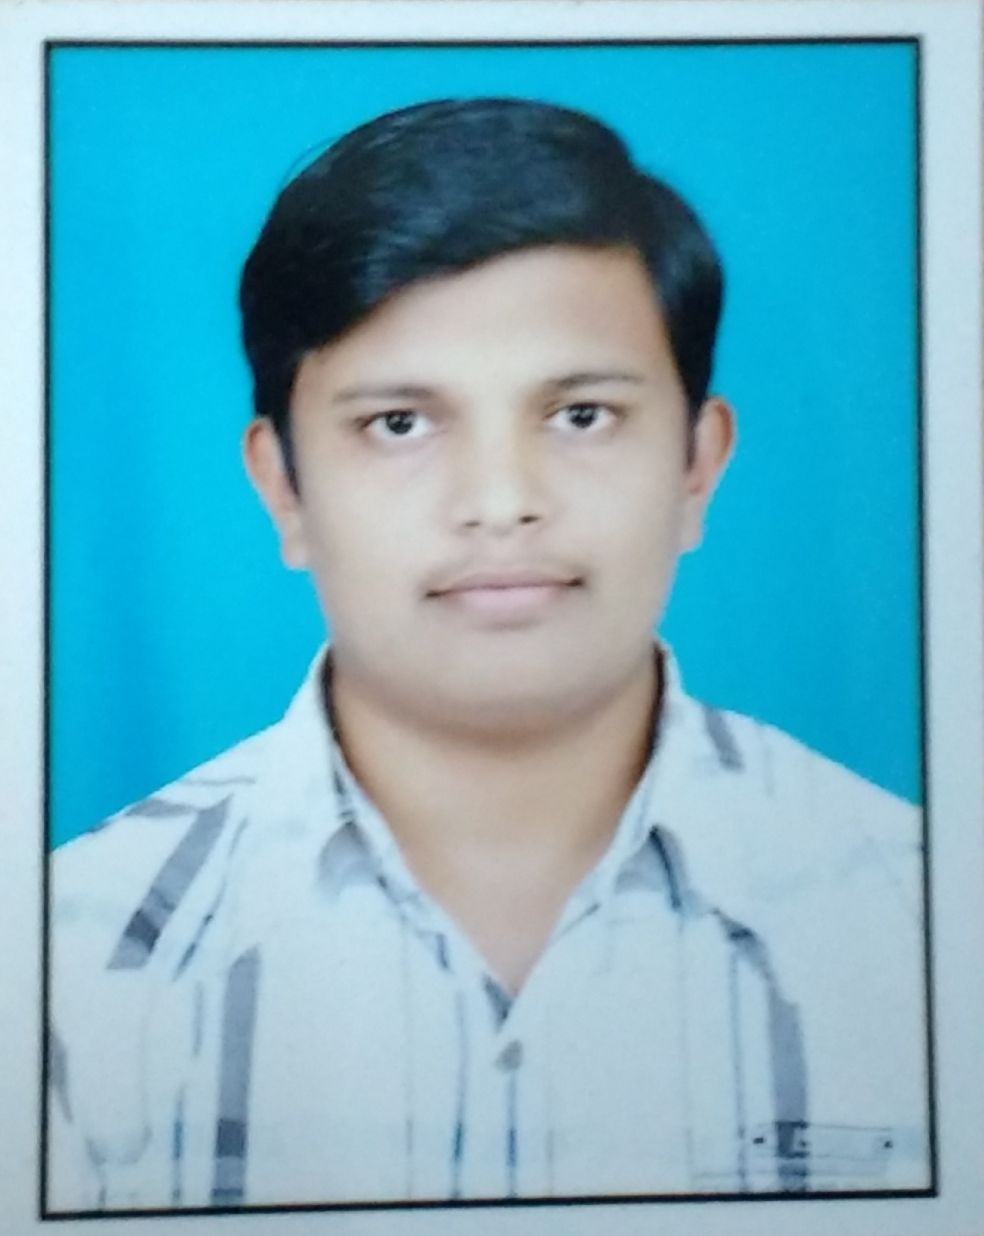
\includegraphics[width=0.2\linewidth,angle=+0]{F:/pritish_photo.jpg}
	\label{fig:pritish_photo}
	\end{flushright}
\end{figure}
\vspace{-4ex}
\begin{flushleft}
\textbf{OBJECTIVE}: To prove myself as a good engineer and be resourceful to the society and to the workplace. }
\end{flushleft}
\begin{flushleft}
\caption{\textbf{EDUCATION:}}\vspace{2ex}
\begin{tabular}{|l|c|c|c|c|r|}  \hline
Degree & College/School & University & Passing Year &  Percentage\\ \hline
B.Tech & Walchand COE, & Shivaji & 2017 & 8.61\\ 
Electrical & Sangli & University & & (CPI) \\ \hline
\end{tabular}
\end{flushleft}
\begin{flushleft}
\textbf{PROJECTS:}
\end{flushleft}
\begin{enumerate}
\item Electrical parameters measurement and protection unit under the guidance of Dr. A P Vaidya
\item Automatic lighting control using instrumentation amplifier.
\item Automatic roof control using water sensor.
\item Image processing based autonomous robot using camera for eYRC+, held by IIT Bombay. 
\end{enumerate}
\begin{flushleft}
\textbf{TRAINING AND INTERNSHIP :}
\begin{itemize}
\item Industrial Training at �Traction Machine Workshop, Nashik�, from 16th July 2015
to 25th July 2015.
\item Industrial Training at �Nashik Thermal Power Station (NTPS), Nashik�, 2015.
\end{itemize}
\end{flushleft}
\begin{flushleft}
\textbf{RESEARCH AND PUBLICATIONS:}\\
1.
\end{flushleft}
\begin{flushleft}
\textbf{TECHNICAL SKILLS : }
\begin{itemize}
\item \textbf{Softwares known:} Microsoft Office 2010, Turbo C, Python(novice), Matlab 2013b, Proteus,Labview, Keil UVision, Arduino.
\item PCB designing using Proteus,power system analysis using Mi-power.
\item Power Electronics and Arduino, 8051, Raspberry-Pi micro-controllers.
\end{itemize}
\end{flushleft}
\begin{flushleft}
\textbf{SOFT SKILLS:}
\begin{enumerate}
\item Multitasking.
\item Teamwork. 
\item Value-maker.
\end{enumerate}
\begin{flushleft}
\textbf{EXTRA CURRICULAR ACTIVITIES :}
\begin{itemize}
\item Member Of Electrical Engineering Students Association (EESA).
\item Playing Cricket.
\end{itemize}
\end{flushleft}
\textbf{CO-CURRICULAR ACTIVITIES : }
\begin{enumerate}
\item \textbf{Winner} in the event Courier Services in e-Yantra+ 2016, a national level robotics competition held by IIT-Bombay.
\item \textbf{Winner} in the event Masterminds in TECHNOCRAT 2014, a state level technical symposium by EESA.
\item \textbf{Runner-up} in the event Stormkries in TECHNOCRAT 2015, a state level technical symposium by EESA.
\item \textbf{Workshops Attended}\\ 1. PLC and SCADA held by ETA (Educate to Automate).\\
\end{enumerate}
\textbf{PERSONAL DETAILS:}\\
\vspace{2ex}
Father's Name : Prakash Raghunath Salunke\\
Mother's Name : Priya Prakash Salunke\\
Birth date : 5th June, 1995\\
Gender : Male\\
Nationality : Indian\\
Languages known : English, Marathi(mother tongue), Hindi\\
\vspace{5ex}
\textbf{Declaration:}\\The above information is true to the best of my knowledge and belief.\\
\vspace{5ex}
\textbf{Date:} 22nd May 2016
\end{flushleft}
\end {document}
